\documentclass{report}
\usepackage{graphicx}
\newcommand{\documentname}{paper~}
\newcommand{\match}{{\tt match}~}
\newcommand{\apj}{ApJ}
\newcommand{\apjs}{ApJS}
\newcommand{\apjl}{ApJL}
\newcommand{\aj}{AJ}
\newcommand{\mnras}{MNRAS}
\newcommand{\mnrassub}{MNRAS accepted}
\newcommand{\aap}{A\&A}
\newcommand{\aaps}{A\&AS}
\newcommand{\araa}{ARA\&A}
\newcommand{\nat}{Nature}
\newcommand{\physrep}{PhR}
\newcommand{\pasp}{PASP}
\newcommand{\pasj}{PASJ} 
\begin{document}


\subsection*{Some general considerations}
The sizes of the HIP, MIP and LIP in units of the Schwarzchild radius
$R_s=2GM_{BH}/c^2$ are $R_{HIP}= (0.003-2.5)\times 10^3$ $R_S$,
$R_{MIP} = (0.057-4.8)\times 10^2$ $R_S$and $R_{LIP}=(0.25 -
2.8)\times 10^4$ $R_S$. 

Furthermore, following \cite{Krongold2007a} we estimate
the line-of-sight thickness given by $\Delta R\sim N_{H}/n_H$, and the
relative value $\Delta R/R$. Using the approximation for a fully
ionized gas of solar abundance on gets $\Delta R/R=1.23N_H (n_e
R^2)^{-1/2} (n_e)^{-1/2}$. In this case we obtain $(\Delta R/
R)_{HIP}=(0.001-1)\times 10^{-3}$, $(\Delta R/ R)_{MIP}=(0.04-5)\times
10^{-5}$ and $(\Delta R/ R)_{LIP}=(0.2-2)\times 10^{-4}$. 

\subsection*{Implications for AGN feedback models}

Here we comment on the potential implications of the values found for
the warm absorber winds in driving the evolution of its host galaxy
NGC3783. Our objective is not to derive a physical model for the
winds, but instead discuss the values obtained in the context of
recent theoretical developments on the physics of AGN feedback. We
now present three relevant facts derived from our observations to
present this discussion.


The first relevant fact derived from our results is that the location of the
different ionization regions, $R$, are close to the black hole with
distances less than a few thousands $R_S$. This is a hint that the
physics of this region are dominated by winds driven by the accretion
disc around the black hole \cite{Murray1995}. The second fact is that
the sizes of these regions $\Delta R$ with respect to their location
is very narrow, on the order of $\Delta R/R\sim $10$^{-5}$. The third
important fact is that the mean values of the kinetic luminosities and the
momentum fluxes computed over all the lines are on the order of
$\dot{E}_k/L_{\rm bol}= (2-8)\%$ and $\dot{P}/(L_{\rm bol}/c)\sim 0.5
-2 $, this is presented in Figure \ref{fig:ep_values}, where we have
used a value of $L_{\rm bol}=1.5\times 10^{43}$ erg s$^{-1}$
\cite{Netzer2003}. 



Recently \cite{Faucher-Giguere2012} gave an explanation for
the low values of $\Delta R/R$ adducing a physical mechanism where the AGN
blast impacts moderately dense interstellar gas clumps along the line
of sight, fragmenting the clumps and sweeping them along the hot
blast. From these model they predict values for the kinetic
luminosities and the momentum fluxes of the order of $\dot{E}_k/L_{\rm
bol}= (2-5)\%$ and $\dot{P}/(L_{\rm bol}/c)\sim 2-15$. Other models
such as the cold thin shell approximation predict order of magnitude
lower values for the kinetic luminosities. This gives a hint that such
process might be at play in the case of NGC-3783. 

The values we infer for the kinetic luminosities and the momentum flux
are in the ballpark of required values to generate an observable
effect on the evolution of the host galaxy
\cite{DiMatteo2005,Debuhr2012}. If we now consider that the outflow 
are in a energy conserving phase the relationship between the energy
of the inflow wind and the swept up gas follows 

\begin{equation}
\frac{1}{2}\dot{M}_{\rm in}v_{\rm in}^2 \approx \dot{M}_{out}v_{out}^2, 
\end{equation}

where the subscript $in$ refers to the wind input values and $out$ to
the outflow measured by the absorption lines. This means that
roghly half of the kinetic if the input wind is converted into bulk
motion of the setp-up gas  \cite{FaucherGiguere2012}. From that
relatinship on can infer the escaling for the input and outflow
momentum flux $\dot{P}_{out}/\dot{P}_{in}\approx 1/2
v_{in}/v_{out}$. Assuming a value of $v_{in}=0.1c$ and $P_{in}=L_{\rm
  AGN}/c$, we obtain the prediction

\begin{equation}
\frac{\dot{P}}{L_{\rm AGN}/c} = \frac{1}{2}\frac{0.1c}{v_{\rm peak}}.
\end{equation}

In Figure \ref{fig:p_ratio} we plot this prediction as a continuous
line, compared to the values inferred in this paper. We find that
there is a reasonable agreement for the median of the velocities
measured from different features in the absorption spectra. We note
that the same prediction for an energy conserving outflow provides a
good fit to outflow measurements of ultraluminous infrared galaxies
(ULIRGS) and FeLoBALs \cite{FaucherGiguere2012}.

In summary, the results in NGC3783 are consistent with a physical
picture where the warm absorber winds are in a energy conserving phase
dominated by winds of velocities $0.1c$ injected close to the accretion
disc region. Furthermore, the values for the momentum flow and kinetic
luminosities suggest that the outflows will have a noticeable impact
on the evolution of the host galaxy.



\begin{figure}
\begin{center}
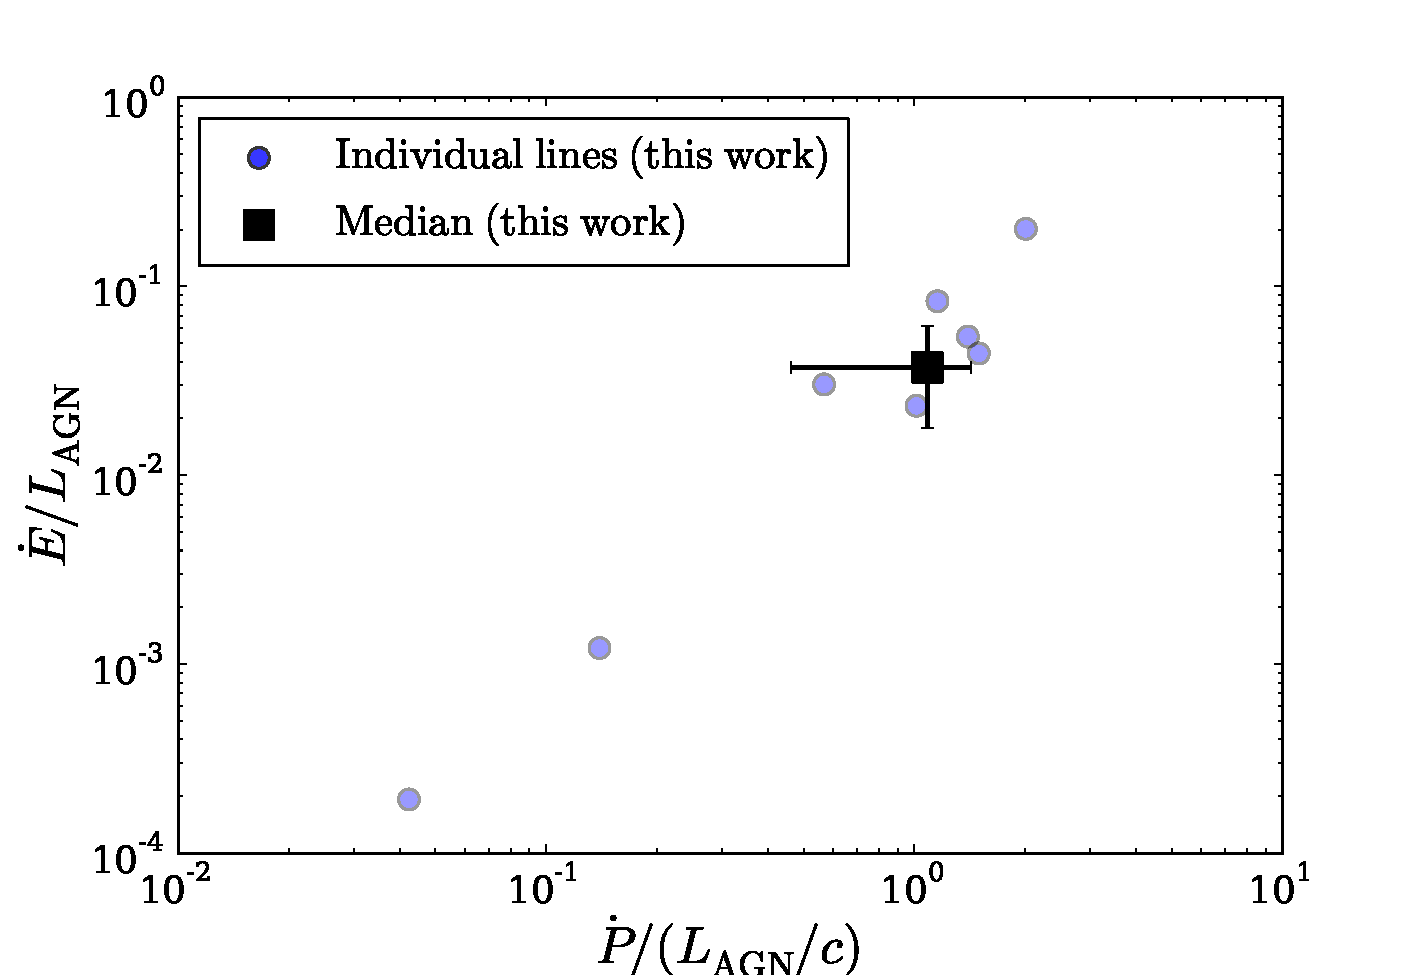
\includegraphics[width=0.9\linewidth,angle=0]{ep_ratio.pdf}
\caption{Kinetic luminosities and momentum flux for the different
  absorption features in the spectrum. The values are consistent with
  theoretical requirements to have an noticeable impact on the
  evolution of the host galaxy as suggested by AGN feedback
  simulations . \label{fig:ep_values}} 
\end{center}
\end{figure}

\begin{figure}
\begin{center}
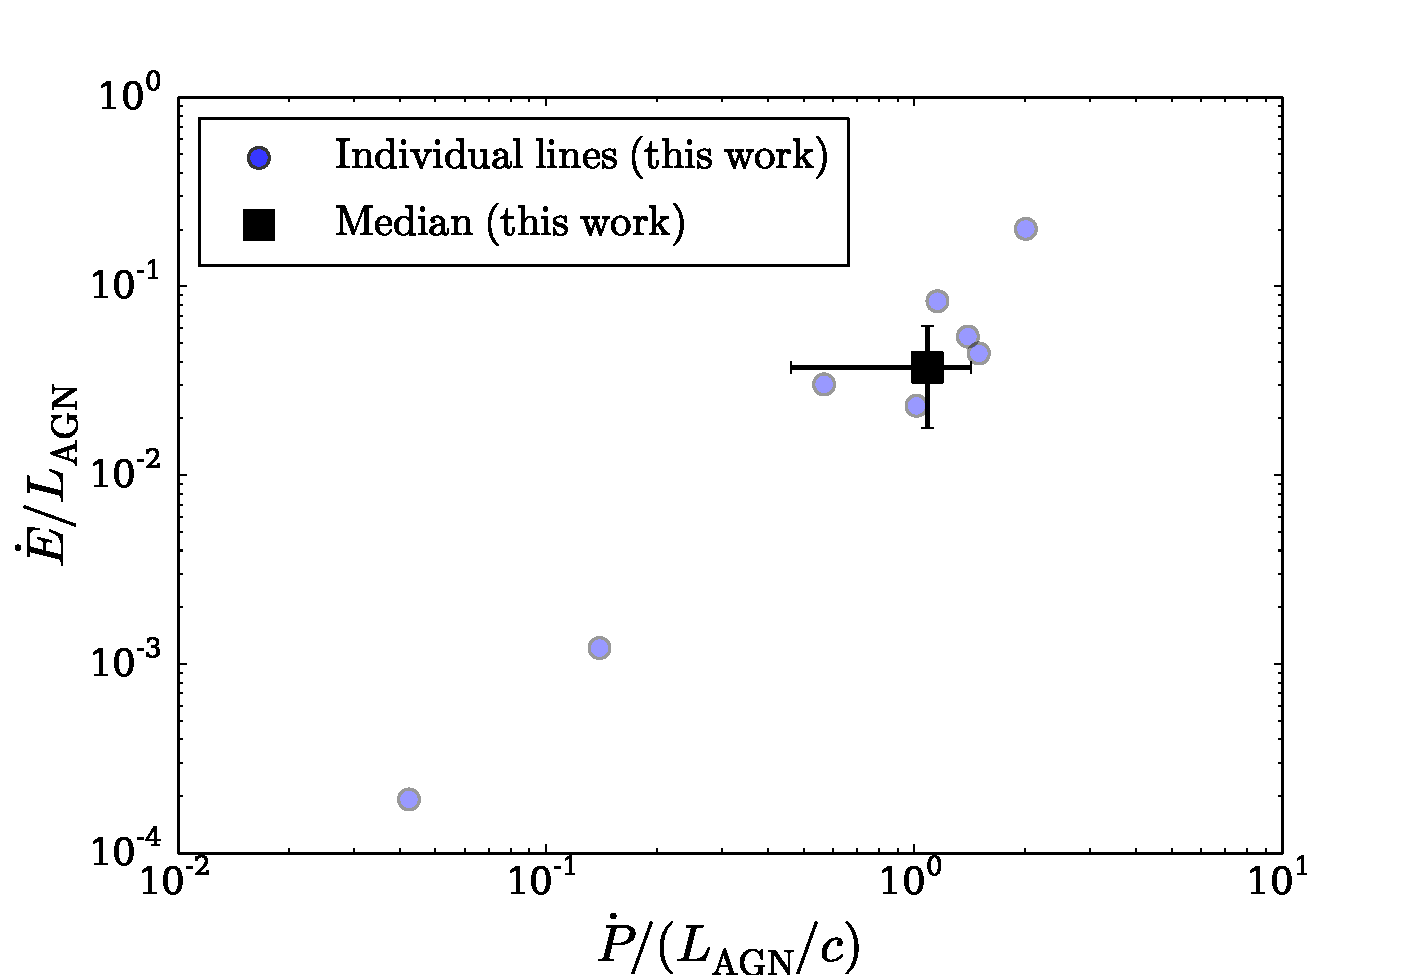
\includegraphics[width=0.9\linewidth,angle=0]{p_ratio_theory.pdf}
\caption{Momentum flux as a function of the peak velocities of
  different absorption features. The line shows the prediction for
  winds in an energy conserving phase that were injected at
  velocities $\sim 0.1c$. \label{fig:p_ratio}}
\end{center}
\end{figure}




\bibliographystyle{plain}
\bibliography{references} 

\end{document}
